\documentclass[10pt]{article}

%Math
\usepackage{amsmath}
\usepackage{amsfonts}
\usepackage{amssymb}
\usepackage{amsthm}
\usepackage{ulem}
\usepackage{stmaryrd} %f\UTF{00FC}r Blitz!

%PageStyle
\usepackage[ngerman]{babel} % deutsche Silbentrennung
\usepackage[utf8]{inputenc} 
\usepackage{fancyhdr, graphicx}
\usepackage[scaled=0.92]{helvet}
\usepackage{enumitem}
\usepackage{parskip}
\usepackage[a4paper,top=2cm]{geometry}
\setlength{\textwidth}{17cm}
\setlength{\oddsidemargin}{-0.5cm}


% Shortcommands
\newcommand{\Bold}[1]{\textbf{#1}} %Boldface
\newcommand{\Kursiv}[1]{\textit{#1}} %Italic
\newcommand{\T}[1]{\text{#1}} %Textmode
\newcommand{\Nicht}[1]{\T{\sout{$ #1 $}}} %Streicht Shit durch
\usepackage{tabto} %Möglichkeit Tabulatoren zu nutzen%

%Arrows
\newcommand{\lra}{\leftrightarrow} 
\newcommand{\ra}{\rightarrow}
\newcommand{\la}{\leftarrow}
\newcommand{\lral}{\longleftrightarrow}
\newcommand{\ral}{\longrightarrow}
\newcommand{\lal}{\longleftarrow}
\newcommand{\Lra}{\Leftrightarrow}
\newcommand{\Ra}{\Rightarrow}
\newcommand{\La}{\Leftarrow}
\newcommand{\Lral}{\Longleftrightarrow}
\newcommand{\Ral}{\Longrightarrow}
\newcommand{\Lal}{\Longleftarrow}

% Code listenings
\usepackage{color}
\usepackage{xcolor}
\usepackage{listings}
\usepackage{caption}
\DeclareCaptionFont{white}{\color{white}}
\DeclareCaptionFormat{listing}{\colorbox{gray}{\parbox{\textwidth}{#1#2#3}}}
\captionsetup[lstlisting]{format=listing,labelfont=white,textfont=white}
\lstdefinestyle{JavaStyle}{
 language=Java,
 basicstyle=\footnotesize\ttfamily, % Standardschrift
 numbers=left,               % Ort der Zeilennummern
 numberstyle=\tiny,          % Stil der Zeilennummern
 stepnumber=5,              % Abstand zwischen den Zeilennummern
 numbersep=5pt,              % Abstand der Nummern zum Text
 tabsize=2,                  % Groesse von Tabs
 extendedchars=true,         %
 breaklines=true,            % Zeilen werden Umgebrochen
 frame=b,         
 %commentstyle=\itshape\color{LightLime}, Was isch das? O_o
 %keywordstyle=\bfseries\color{DarkPurple}, und das O_o
 basicstyle=\footnotesize\ttfamily,
 stringstyle=\color[RGB]{42,0,255}\ttfamily, % Farbe der String
 keywordstyle=\color[RGB]{127,0,85}\ttfamily, % Farbe der Keywords
 commentstyle=\color[RGB]{63,127,95}\ttfamily, % Farbe des Kommentars
 showspaces=false,           % Leerzeichen anzeigen ?
 showtabs=false,             % Tabs anzeigen ?
 xleftmargin=17pt,
 framexleftmargin=17pt,
 framexrightmargin=5pt,
 framexbottommargin=4pt,
 showstringspaces=false      % Leerzeichen in Strings anzeigen ?        
}

%Config
\renewcommand{\headrulewidth}{0pt}
\setlength{\headheight}{15.2pt}

%Metadata
\fancyfoot[C]{If you use this documentation for a exam, you should offer a beer to the authors!}
\title{
	\vspace{5cm}
	Verteilte Systeme - Zusammenfassung
}
\author{Jan Fässler \& Chregi Glatthard}
\date{4. Semester (FS 2013)}


% hier beginnt das Dokument
\begin{document}

% Titelbild
\maketitle
\thispagestyle{fancy}

\newpage

% Inhaltsverzeichnis
\pagenumbering{Roman}
\tableofcontents	  	


\newpage
\setcounter{page}{1}
\pagenumbering{arabic}

% Inhalt Start

\section{Networking}
\subsection{InetAddress}
\subsubsection*{Static factory methods}
\begin{itemize}
	\item getByName(String name)
	\item getByAddress (4/16 bytes)
	\item getAllByName(String host)
	\item getLocalHost()
\end{itemize}
\subsubsection*{Instance methods}
\begin{itemize}
	\item byte[] getAddress()
	\item String getHostAddress()
	\item String getHostName()
	\item String getCanonicalHostName()
	\item boolean isReachable(int timeout)
	\item boolean isMulticastAddress()
\end{itemize}
\subsection{Network Interfaces}
\begin{lstlisting}[language=Java, caption=Network Interfaces and its addresses, style=JavaStyle]
public static void main(String[] args) throws SocketException {
	Enumeration<NetworkInterface> interfaces = NetworkInterface.getNetworkInterfaces();
	while(interfaces.hasMoreElements()){
		NetworkInterface intf = interfaces.nextElement();
		Syst	em.out.print(intf.getName());
		System.out.println(" ["+intf.getDisplayName()+"]");
		Enumeration<InetAddress> adr = intf.getInetAddresses();
		while(adr.hasMoreElements()){
			System.out.println("\t" + adr.nextElement());
		}
		byte[] hardwareAddress = intf.getHardwareAddress();
	}
}
\end{lstlisting}
\subsection{Sockets}
Abstraction through which an application may send and receive data through the network. A Socket is identified by Hostname/IP and port number.
\begin{description}
	\item[Stream Sockets] \hfill
	\begin{itemize}
		\item Use TCP as end-to-end protocol
		\item Provide a reliable byte-stream
		\item Connection oriented: Socket represents one end of a TCP connection
	\end{itemize}
	\item[Datagaram Sockets] \hfill 
	\begin{itemize}
		\item Use UDP as protocol
		\item Not connection oriented, not reliable
	\end{itemize}
\end{description}
\subsubsection{Controlling Socket Behaviors}
\begin{description}
	\item[Blocking \& Timeouts] \hfill 
	\begin{description}
		\item[ServerSocket.accept / InputStream.read] \hfill \\
			read or accept call will not block for more than a fixed number of msec otherwise, InterruptedIOException is thrown (get/setSoTimeout(int timeout))
		\item[Socket constructor] \hfill \\
			Uses a system-defined timeout, cannot be changed by Java API (Solution: use connect)
		\item[OutputStream.write] \hfill \\
			Cannot be interrupted / caused to time-out by Java API
	\end{description}
	\item[Keep-Alive] \hfill
	\begin{itemize}
		\item TCP provides a keep-alive mechanism
		\item Probe messages are sent after a certain time
		\item Application only sees keep-alive working if the probes fail!
		\item Per default keep-alive is disabled
		\item Default timeout: 2h (7200 secs)
	\end{itemize}
	\item[Send / Receive Buffer Size] \hfill
	\begin{itemize}
		\item When a Socket is created, the OS must allocate buffers to hold incoming \& outgoing data
		\item Receive buffer size may also be specified on server socket (for accepted
sockets which immediately receive data)
	\end{itemize}
	\item[No Delay] \hfill
	\begin{itemize}
		\item TCP tries to avoid sending small packets
		\item Buffers data until it has more to send, combines small packets with larger ones
		\item Necessary if application has to be efficient
		\item Default: false
	\end{itemize}
\end{description}
\subsubsection{Closing Connections}
\begin{description}
	\item[close()] \hfill 
	\begin{itemize}
		\item Once an endpoint (client or server) closes the socket, it can no longer send or receive data	
		\item Close can only be used to signal the other end that the caller is completely finished communicating
	\end{itemize}
	\item[shutdownOutput()] \hfill
	\begin{itemize}
		\item Closes output-stream, no more data can be may be written (IOException)
		\item All data written before shutdownOutput can be read by receiver
	\end{itemize}
	\item[shutdownInput()] \hfill
	\begin{itemize}
		\item Closes the input stream
		\item Any undelivered data is (silently) discarded, read operations will return -1
	\end{itemize}
	\item[s.close() / s.shutdownOutput()] \hfill
	\begin{itemize}
		\item Data may still be waiting to be delivered to the other side
		\item By default, socket tries to deliver remaining data, but if socket crashes, data may be lost without notification to sender (as close returns immediately)
	\end{itemize}
\end{description}
\subsubsection{User Datagram Protocol}
\begin{itemize}
	\item UDP allows to address applications over ports
	\item UDP adds another layer of addressing (ports) to that of IP
	\item UDP detects some form of data corruption that may occur in transit and discards corrupted messages
	\item UDP retains message boundaries
\end{itemize}

\newpage
\section{Internet}
\subsection{Protocol}
\begin{description}	
	\item[GET] \hfill
	\begin{itemize}
		\item Access of content from the server
		\item Idempotent, i.e. the side effects of N>0 identical requests is the same as for a single request ( f(f(x)) = f(x) )
	\end{itemize}
	\item[POST] \hfill \\
		Comparable to GET but Method must not necessarily be idempotent and Request data is transferred in the body of the request
	\item[HEAD] \hfill
	\begin{itemize}
		\item Identical to GET, except that the server must not return the body
		\item Can be used to request meta information (headers) about the resource
	\end{itemize}
	\item[OPTIONS (1.1)] \hfill \\
		Returns information about the communication options available on the specified resource (or on the server in general if request URI=*)
	\item[PUT (1.1)] \hfill \\
		Stores a web page on the server (rarely implemented)
	\item[DELETE (1.1)] \hfill \\
		Removes a web resource from the servver (rarely implemented)
	\item[TRACE (1.1)] \hfill \\
		Returns the request as it was accepted by server ($\Ra$ debugging)
	\item[CONNECT (1.1)] \hfill \\
		Implemented by Proxy Server capable to provide an SSL tunnel
\end{description}
\subsubsection{Response Codes}
\begin{description}
	\item[200-299: Success] \hfill
	\begin{itemize}
		\item[200] OK
		\item[201] Created
		\item[202] Accepted
	\end{itemize}
	\item[300-399: Redirections] \hfill
	\begin{itemize}
		\item[300] Multiple Choices
		\item[301] Moved Permanently
		\item[302] Found
		\item[303] See Other (e.g. after POST)
		\item[304] Not Modified
		\item[305] Use Proxy
		\item[307] Temporary Redirect
	\end{itemize}
	\item[400-499: Client Error] \hfill
	\begin{itemize}
		\item[400] Bad Request
		\item[401] Unauthorized
		\item[402] Payment Required
		\item[403] Forbidden
		\item[404] Not Found
		\item[405] Method Not Allowed
		\item[407] Proxy Authentication Required
		\item[408] Request Time-out
		\item[411] Length Required
		\item[413] Request Entity Too Large
		\item[414] Request-URI Too Large
		\item[415] Unsupported Media Type
	\end{itemize}
	\item[500-599: Server Error] \hfill
	\begin{itemize}
		\item[500] Internal Server Error
		\item[501] Not Implemented
		\item[503] Service Unavailable
		\item[505] HTTP Version not supported
	\end{itemize}
\end{description}
\subsection{Request Headers}
\begin{description}
	\item[Host] server host 
	\item[Referer] host from which the request is initiated
	\item[Accept] data types supported by the client 
	\item[Accept-Language] language supported by client
	\item[Accept-Encoding] encodings supported by client, e.g. gzip or deflate
	\item[User-Agent] browser details, supplies server with information about the type of browser making the request
	\item[Connection: Keep-Alive] browser is requesting the use of persistent TCP connections
\end{description}
\subsection{Response Headers}
\begin{description}
	\item[Content-Type] MIME-Type of content
	\item[Content-Length] size of body (in bytes)
	\item[Content-Encoding] compression algorithms
	\item[Location] used by redirections
	\item[Date] timestamp when the response was created 
	\item[Last-Modified] modification date of resource (assumed by server) 
	\item[Expires] date after which the result is considered stale 
	\item[Server] information about the server
	\item[Transfer-Encoding] specifies type of transformation
	\item[Cache-Control] information about cache handling (e.g. no-cache disables caching)
	\item[WWW-Authenticate] information about authentication method
\end{description}
\subsection{Servlet}
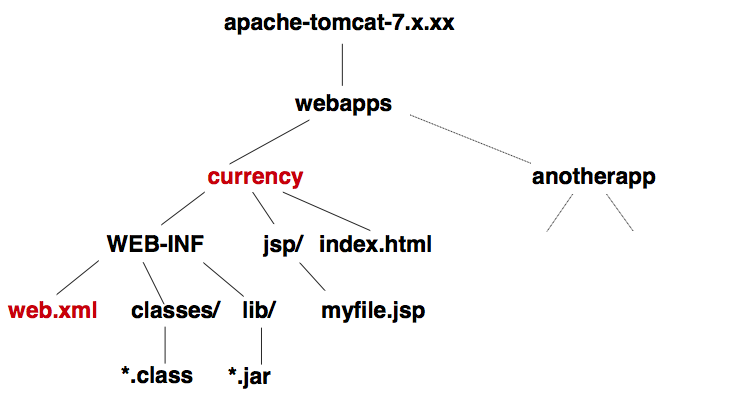
\includegraphics[scale=0.5]{tomcat-structure.png}
\begin{lstlisting}[language=Java, caption=Servlet Example, style=JavaStyle]
public class Converter extends HttpServlet {
	public void doGet(HttpServletRequest request, HttpServletResponse response) throws IOException {
		response.setContentType("text/html");
		PrintWriter out = response.getWriter();
		String amount = request.getParameter("amt"); 
		String from = request.getParameter("from"); 
		String to = request.getParameter("to"); 
		String res = computeResult(amount, from, to);
		out.println("<html>\n<body bgcolor=\"white\">"); 
		out.println("<h1>Currency Converter</h1>"); 
		out.println(amount + " " + from + " = " + res);
		out.println("</body>\n</html>");
	}
	String computeResult(String amount, String from, String to){...}
}
\end{lstlisting}
\begin{lstlisting}[language=Java, caption=web.xml, style=JavaStyle]
<?xml version="1.0" encoding="ISO-8859-1"?>
<web-app xmlns="http://java.sun.com/xml/ns/javaee" xmlns:xsi="http://www.w3.org/2001/XMLSchema-instance" xsi:schemaLocation="http://java.sun.com/xml/ns/javaee http://java.sun.com/xml/ns/javaee/web-app_3_0.xsd" version="3.0">
    <servlet>
        <servlet-name>CurrencyConverter</servlet-name>
        <servlet-class>ch.fhnw.ds.Converter</servlet-class>
    </servlet>
    <servlet-mapping>
        <servlet-name>CurrencyConverter</servlet-name>
		<url-pattern>/convert</url-pattern>
	</servlet-mapping>
</web-app>
\end{lstlisting}

\section{Webservices}
\subsection{XML-RPC}

simples RPC Protokoll über HTTP, benötigt keine lange Einarbeitungszeit
\subsubsection{Primitive Datentypen}
\begin{itemize}
\item int, i4 \tab signed 32bit Integer
\item string \tab ASCII string (no latin1)
\item boolean \tab either 0 or 1
\item double \tab double-precision floating point number
\item dateTime.iso8601 \tab z.B. 20050717T14:08:14
\item base64 \tab raw binary data, base64 encoded
\end{itemize}

\begin{lstlisting}[language=Java, caption=Beispiele, style=JavaStyle]
<i4>13</i4>
<boolean>0</boolean>
\end{lstlisting}

\subsubsection{Structs}
\begin{itemize}
\item Struct enthält Members mit Name und Wert.
\item können rekursiv sein (Structs die Structs enthalten)
\end{itemize}

\begin{lstlisting}[language=Java, caption=Struct Beispiel, style=JavaStyle]
<i4>13</i4>
<struct> 
  <member> 
    <name>from</name> 
    <value><i4>-5</i4></value> 
  </member> 
  <member> 
    <name>to</name> 
    <value><i4>5</i4></value> 
  </member>
</struct>
\end{lstlisting}

\subsubsection{Arrays}
\begin{itemize}
\item Element-Typen können gemischt werden
\end{itemize}

\begin{lstlisting}[language=Java, caption=Array, style=JavaStyle]
<array>
 <data>
  <value><i4>-5</i4></value>
  <value><string>44</string></value>
  <value><boolean>1</boolean></value>
 </data> 
</array>
\end{lstlisting}

\subsubsection{XML-RPC Request}
\begin{lstlisting}[language=Java, caption=Method Call, style=JavaStyle]
<?xml version="1.0" encoding="UTF-8"?>
<methodCall>
  <methodName>Echo.getEcho</methodName>
    <params>
      <param>
        <value>World</value>
      </param>
    </params>
</methodCall>
\end{lstlisting}

\subsubsection{XML-RPC Response}
\begin{lstlisting}[language=Java, caption=Single Result, style=JavaStyle]
<?xml version="1.0" encoding="UTF-8"?>
<methodResponse>
  <params>
    <param>
      <value>Hello World, welcome to XML-RPC</value>
    </param>
  </params>
</methodResponse>
\end{lstlisting}
Als Resultat kann nur ein Wert zurückkommen, dieser kann jedoch auch ein Struct oder ein Array sein.

\begin{lstlisting}[language=Java, caption=Fault Result, style=JavaStyle]
<?xml version="1.0" encoding="UTF-8"?>
<methodResponse>
  <fault>
    <value>
      <struct>
        <member>
          <name>faultCode</name>
          <value><i4>0</i4></value>
        </member>
        <member>
          <name>faultString</name>
          <value>No such handler: Echo.foo</value>
        </member>
      </struct>
    </value>
  </fault>
</methodResponse>
\end{lstlisting}

\subsubsection{Apache XML-RPC Sample Server}
\lstinputlisting[language=java,caption=Sample Server,style=JavaStyle]{code/ApacheXML-RPC-Server1.class}

\lstinputlisting[language=java,caption=Handler Class Server,style=JavaStyle]{code/ApacheXML-RPC-Server2.class}

Nur Instanzmethoden der Handlerklasse sind zugreifbar. Keine void Methoden. Public Default Constructor zwingend.

\subsubsection{Apache XML-RPC Client}
\lstinputlisting[language=java,caption=Handler Class Server,style=JavaStyle]{code/ApacheXML-RPC-Client.class}


\subsection{SOAP}
\subsubsection{WSDL (Web Services Description Language)}
früher Web Services Definition Language
\subsubsection{JAX-WS (Java API for XML Web Services}
\begin{itemize}
\item Java-API zum Erstellen von Webservices
\item Benutzt Annotationen um Entwicklung und Deployment von Clients und Service-Endpunkten zu vereinfachen
\item Kommunikation über SOAP
\item unterstützt erst WSDL 1.1
\end{itemize}

\subsection{XML-RPC vs SOAP}

\section{REST}

% Inhalt Ende 
\end{document} 